\chapter{Supplementary information to \Chapref{STD_paper}}
\label{chap:Appendix_STD}

\bigskip
\medskip
\begin{center}

\noindent{\Large \bf Mammalian morphological diversity does not increase in response to the Cretaceous-Paleogene mass extinction and the extinction of the (non-avian) dinosaurs} \\
\bigskip
\end{center}

\section{Rarefied results for each datasets.}
This section contains the results of the rarefied analyses of disparity through time for Mammaliaformes and Eutheria.
We ran the rarefaction analysis to test whether disparity might be higher in subsamples with more phylogenetic elements simply because there are more taxa represented (see Chapter \ref{chap:STD_paper}, section \ref{testing_disparity} for details).
For each dataset, we reduced the number of tips and nodes to the strict minimum (i.e. three tips or nodes in each subsample) and to the minimum number of Mammaliaformes in the subsamples from 170 Ma to the present (eight tips or nodes in each subsample; as in Fig. \ref{fig:Fig_Rar_results}).
Note that these analyses do not change our results, see Tables \ref{tab:Tab_results} and \ref{tab:Tab_rare} in Chapter \ref{chap:STD_paper} for more details.

\begin{figure}
\centering
    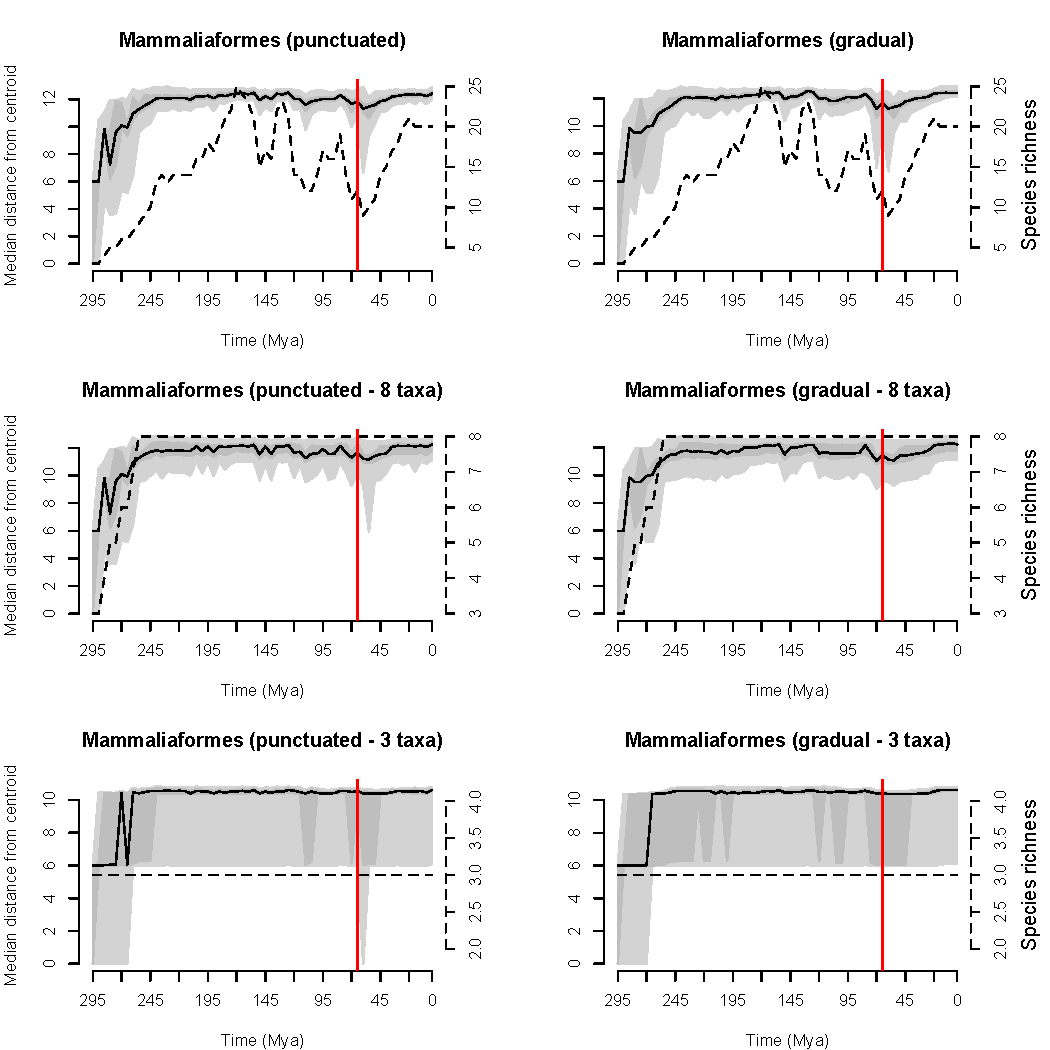
\includegraphics[keepaspectratio=true]{Supplementaries/Figures/STD/Slater_full.pdf}
\caption[Mammaliaformes disparity (rarefied)]{Observed and rarefied variation of disparity through time among Mammaliaformes with a punctuated or gradual evolution model. The x axis represents time in millions of years before the present (Ma). The y axis represents disparity, measured as the median distance between the centroid of the ordinated space and the tips/nodes in each time subsample. The solid black lines show the mean disparity estimated from 1000 bootstrapped pseudoreplicates and confidence intervals (CI) are represented by the grey polygons (50\% CI in dark grey and 95\% CI in light grey). The dashed line and the right hand axis represents the number of tips/nodes in each time slice. The red vertical line indicates the Cretaceous-Paleogene (K-Pg) boundary (66 Ma). Note that scale bars differ among panels.}
\label{Supp_Mammaliaformes_rarefied}
\end{figure}

\begin{figure}
\centering
    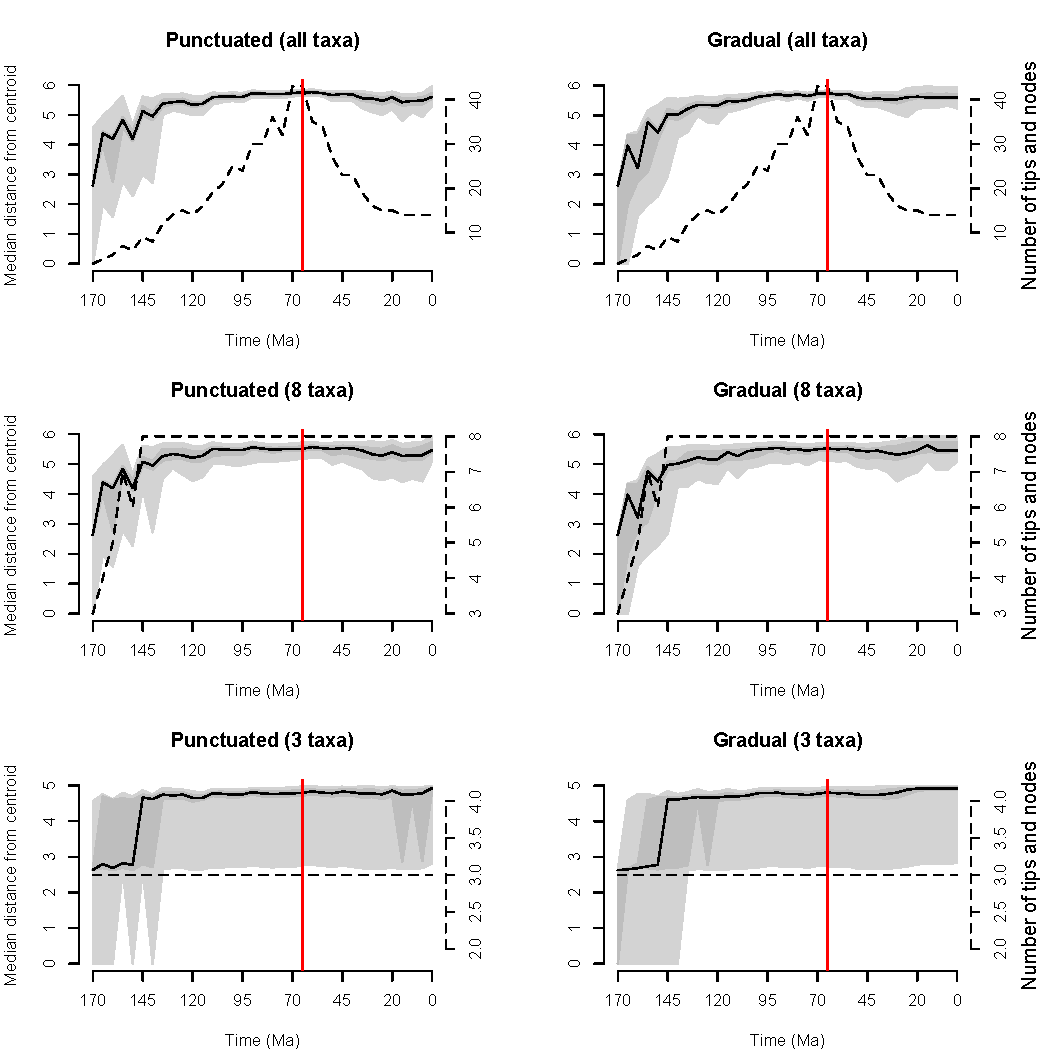
\includegraphics[keepaspectratio=true]{Supplementaries/Figures/STD/Rarefaction-beck.pdf}
\caption[Eutheria disparity (rarefied)]{Variations of disparity through time among Eutheria with a punctuated or gradual evolution model for different number of taxa (rarefaction). The x axis represents time in millions of years before the present (Ma). The y axis represents disparity, measured as the median distance between the centroid of the ordinated space and the tips/nodes in each time subsample. The solid black lines show the mean disparity estimated from 1000 bootstrapped pseudoreplicates and confidence intervals (CI) are represented by the grey polygons (50\% CI in dark grey and 95\% CI in light grey). The dashed line and the right hand axis represents the number of tips/nodes in each time slice. The red vertical line indicates the Cretaceous-Paleogene (K-Pg) boundary (66 Ma). Note that scale bars differ among panels.}
\label{Supp_Eutheria_rarefied}
\end{figure}

\newpage
\section{Comparison of different disparity metrics and time sampling methods.}
This section (Fig. \ref{Supp_disparity_all_Mammaliaformes}, \ref{Supp_disparity_all_Eutheria}, \ref{Supp_disparity_all_Mammaliaformes_rarefied} and \ref{Supp_disparity_all_Eutheria_rarefied}) contains the results of the variation of disparity through time analyses for Mammaliaformes and Eutheria using all the disparity metrics and methods for sampling disparity through time.
The different disparity metrics are the median distance from centroid (see Chapter \ref{chap:STD_paper}, section \ref{disparity_calc}), and the sum and products of ranges and variances of the cladisto-space dimensions \citep{Wills1994}.
The sum and products of ranges and variances are calculated as follows:

\begin{equation}
    \text{Sum of ranges}=\sum{(max(\mathbf{v}_{n})-min(\mathbf{v}_{n}))}
\end{equation}
\begin{equation}
    \text{Sum of variances}=\sum{(\sigma^{2}(\mathbf{v}_{n}))}
\end{equation}
\begin{equation}
    \text{Product of ranges}=\prod{(max(\mathbf{v}_{n})-min(\mathbf{v}_{n}))}
\end{equation}
\begin{equation}
    \text{Product of variances}=\prod{(\sigma^{2}(\mathbf{v}_{n}))}
\end{equation}

\noindent
where $\mathbf{v}_{n}$ is any of the $n$ eigenvectors (i.e. any of the $n$ dimensions of the cladisto-space), $max$ and $min$ are respectively the maximum and minimum values of each eigenvector $\mathbf{v}_{n}$, and $\sigma^{2}$ is the variance of each eigenvector $\mathbf{v}_{n}$. 

The different time sampling methods are as follows:
\begin{enumerate}
\item \textbf{Intervals (tips only)}.
We selected every tip present at every geological stage (i.e. the smaller stratigraphic units) from the early Middle Jurassic (Bajocian, starting at 170.3 Ma) to the present.
We collapsed together every stage containing fewer than three tips so that every time interval contained at least three tips.
Note that some tips were present in multiple stages due to their occurrence data (see Chapter \ref{chap:STD_paper}, section \ref{phylogenies} for details).
\item \textbf{Intervals (tips and nodes)}.
We selected tips and nodes present at every stage from the early Middle Jurassic (Bajocian, starting at 170.3 Ma) to the present.
We collapsed together every stage containing fewer than three elements (tips and/or nodes).
\item \textbf{Slices (punctuated)}.
These are the results presented in the main text where the cladisto-space is sampled every 5 Ma and the mode of evolution between each subsample is assumed to be punctuated (randomly selecting either data from the descendant or the ancestor when slicing through a branch; see Chapter \ref{chap:STD_paper}, section \ref{time_slicing} for details).
\item \textbf{Slices (punctuated: ACCTRAN)}.
Similar to the slices (punctuated) method but data are always selected from the descendant (see Chapter \ref{chap:STD_paper}, section \ref{time_slicing} for details).
\item \textbf{Slices (punctuated: DELTRAN)}.
Similar to the slices (punctuated) method but data are always selected from the ancestor (see Chapter \ref{chap:STD_paper}, section \ref{time_slicing} for details).
\item \textbf{Slices (gradual)}.
These are the results presented in the main text where the cladisto-space is sampled every 5 Ma and the mode of evolution is assumed to be gradual (data is selected from the descendant or the ancestor based on branch length; see Chapter \ref{chap:STD_paper}, section \ref{time_slicing} for details).
\end{enumerate}
We also rarefied both datasets for all the metrics and all the methods using the minimum of three taxa for the interval methods, and eight taxa for the slices methods.

\begin{landscape}
\begin{figure}[!htbp]
\centering
    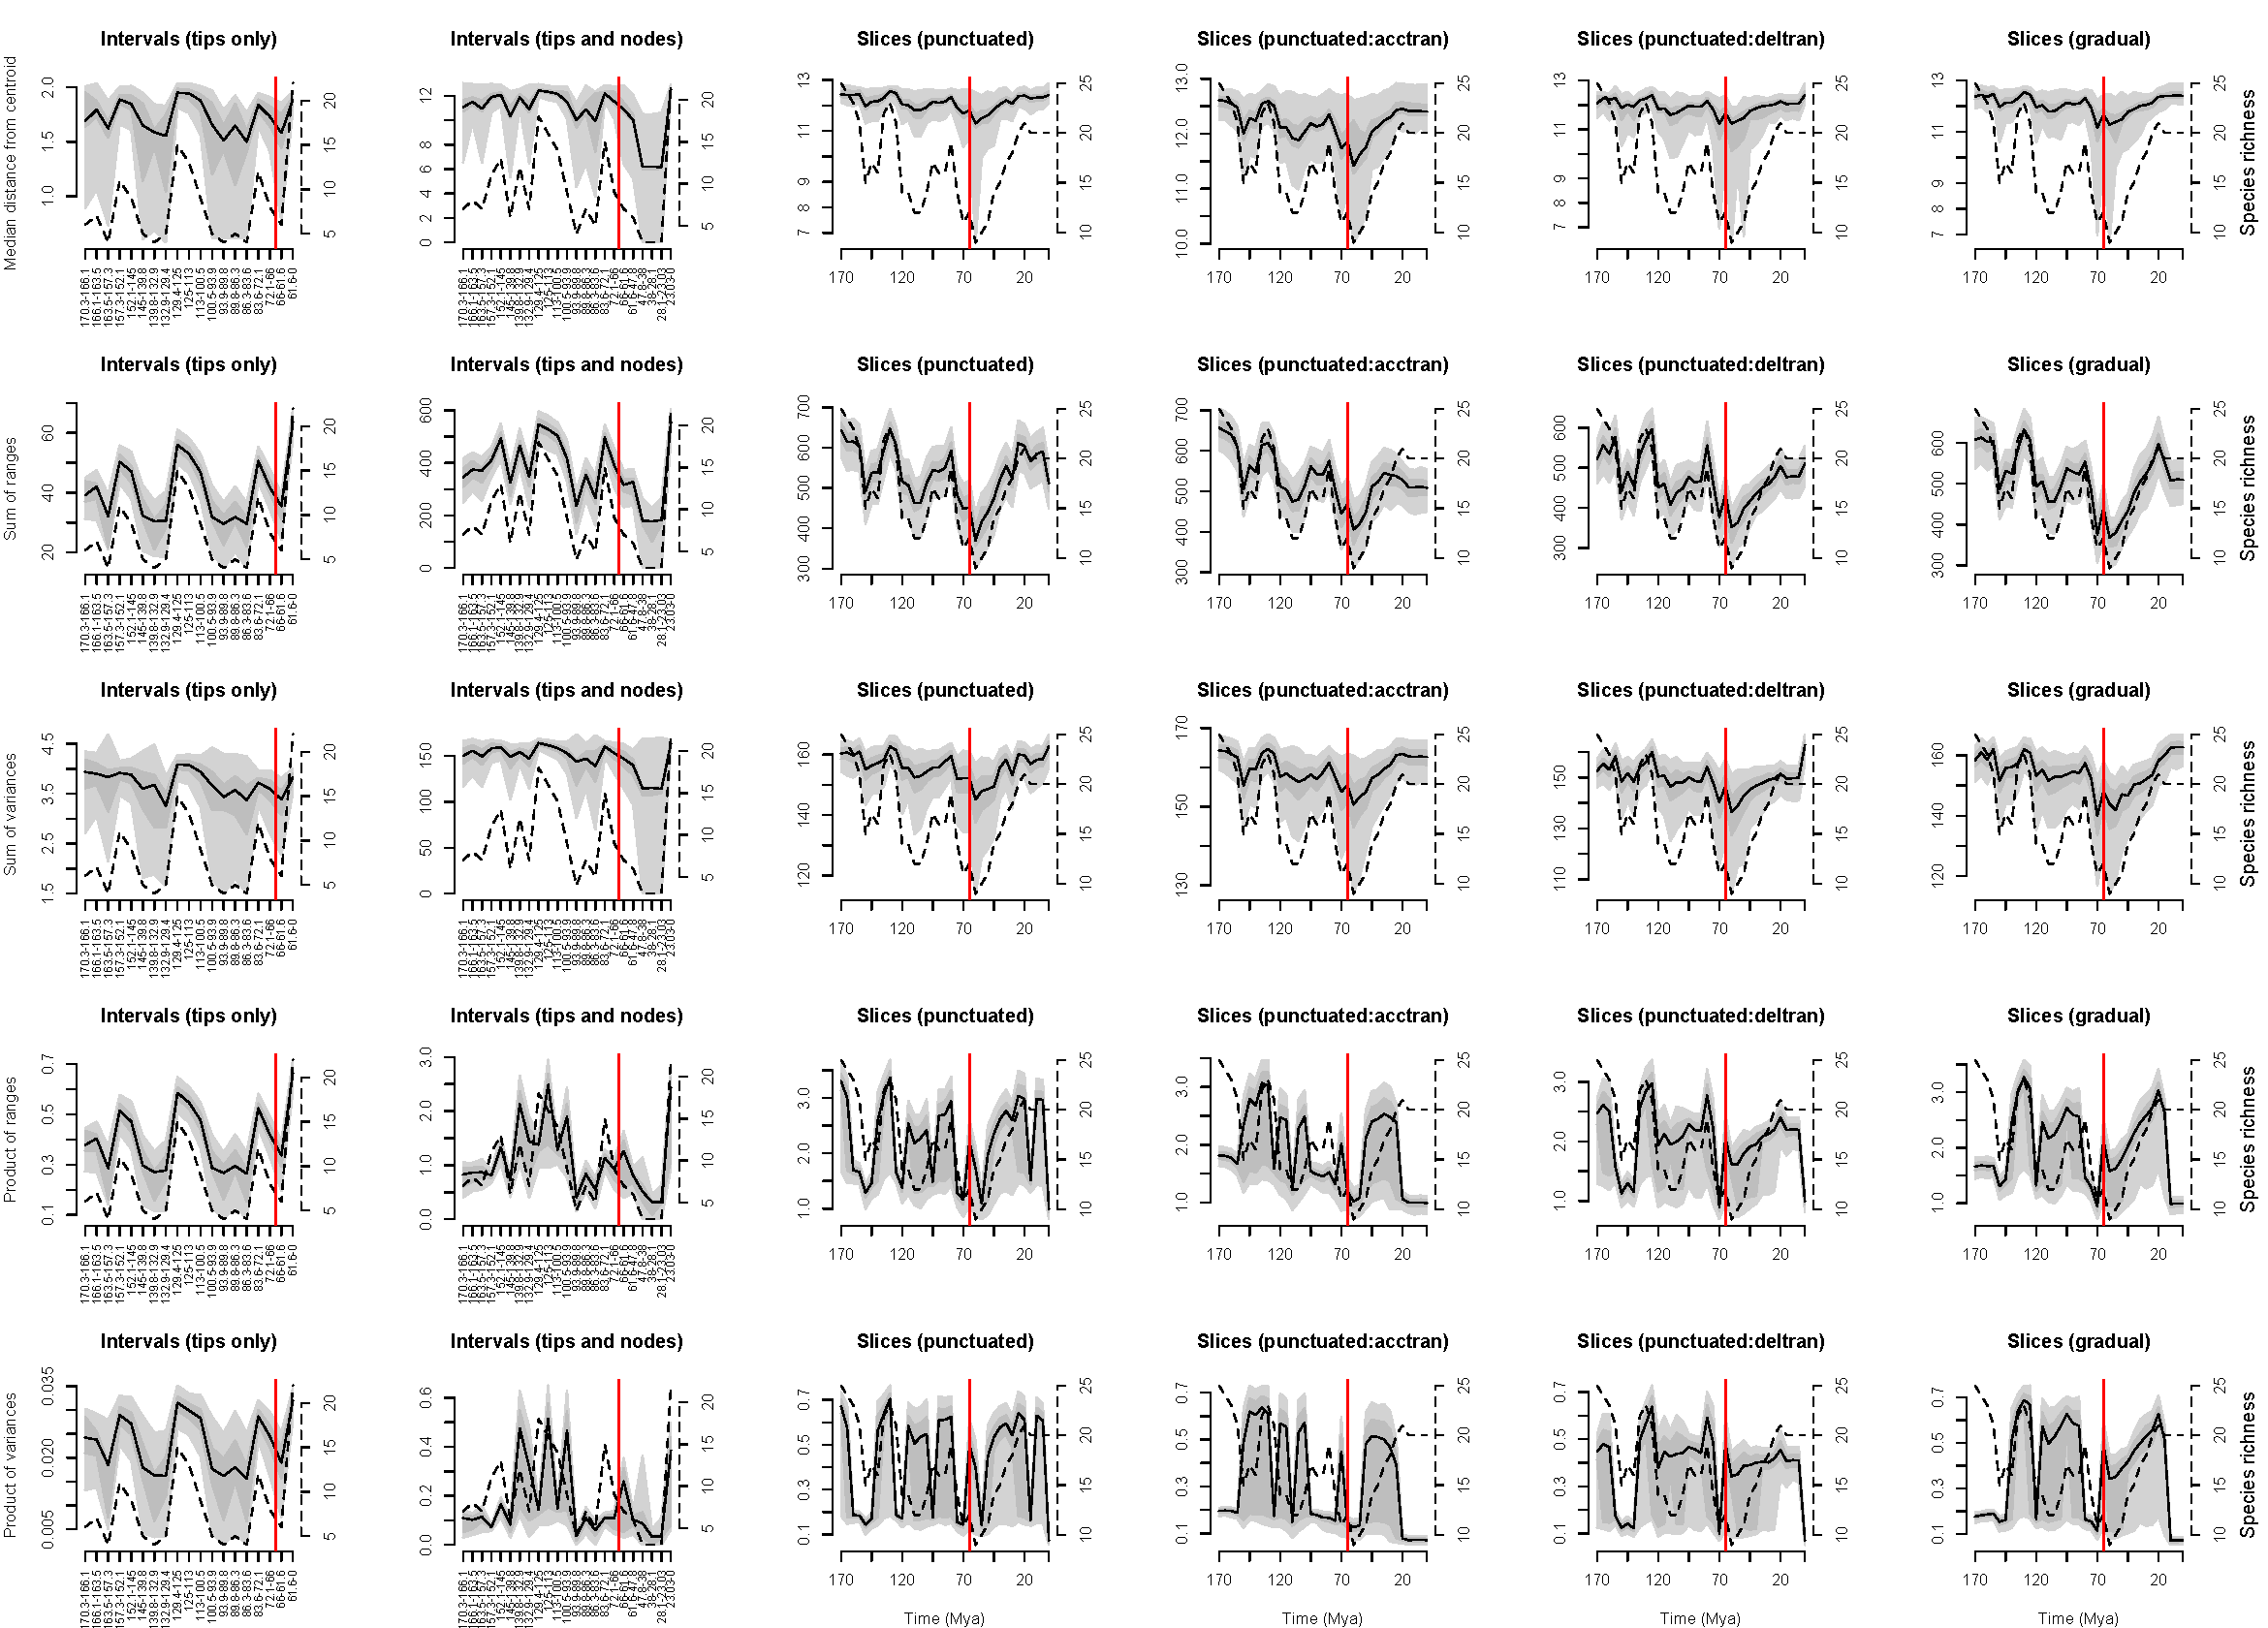
\includegraphics[width=\textwidth,height=\textheight,keepaspectratio]{Supplementaries/Figures/STD/Mammaliaformes_all_methods.pdf}
\caption[Comparison of all the disparity metrics and all the time sampling methods for Mammaliaformes]{Variations in disparity through time among Mammaliaformes with different disparity measurements and methods for sampling disparity through time. The x axis represents time in millions of years before the present (Ma). The y axis represents disparity, measured either as the median distance between the centroid of the ordinated space and the tips/nodes in each time subsample, or the sum and product of ranges and variances of each axis of the cladisto-space. The solid black lines show the mean disparity estimated from 1000 bootstrapped pseudoreplicates and confidence intervals (CI) are represented by the grey polygons (50\% CI in dark grey and 95\% CI in light grey). The dashed line and the right hand axis represents the number of tips/nodes in each time slice. The red vertical line indicates the Cretaceous-Paleogene (K-Pg) boundary (66 Ma). Note that scale bars differ among panels.}
\label{Supp_disparity_all_Mammaliaformes}
\end{figure}
\end{landscape}

\begin{landscape}
\begin{figure}[!htbp]
\centering
    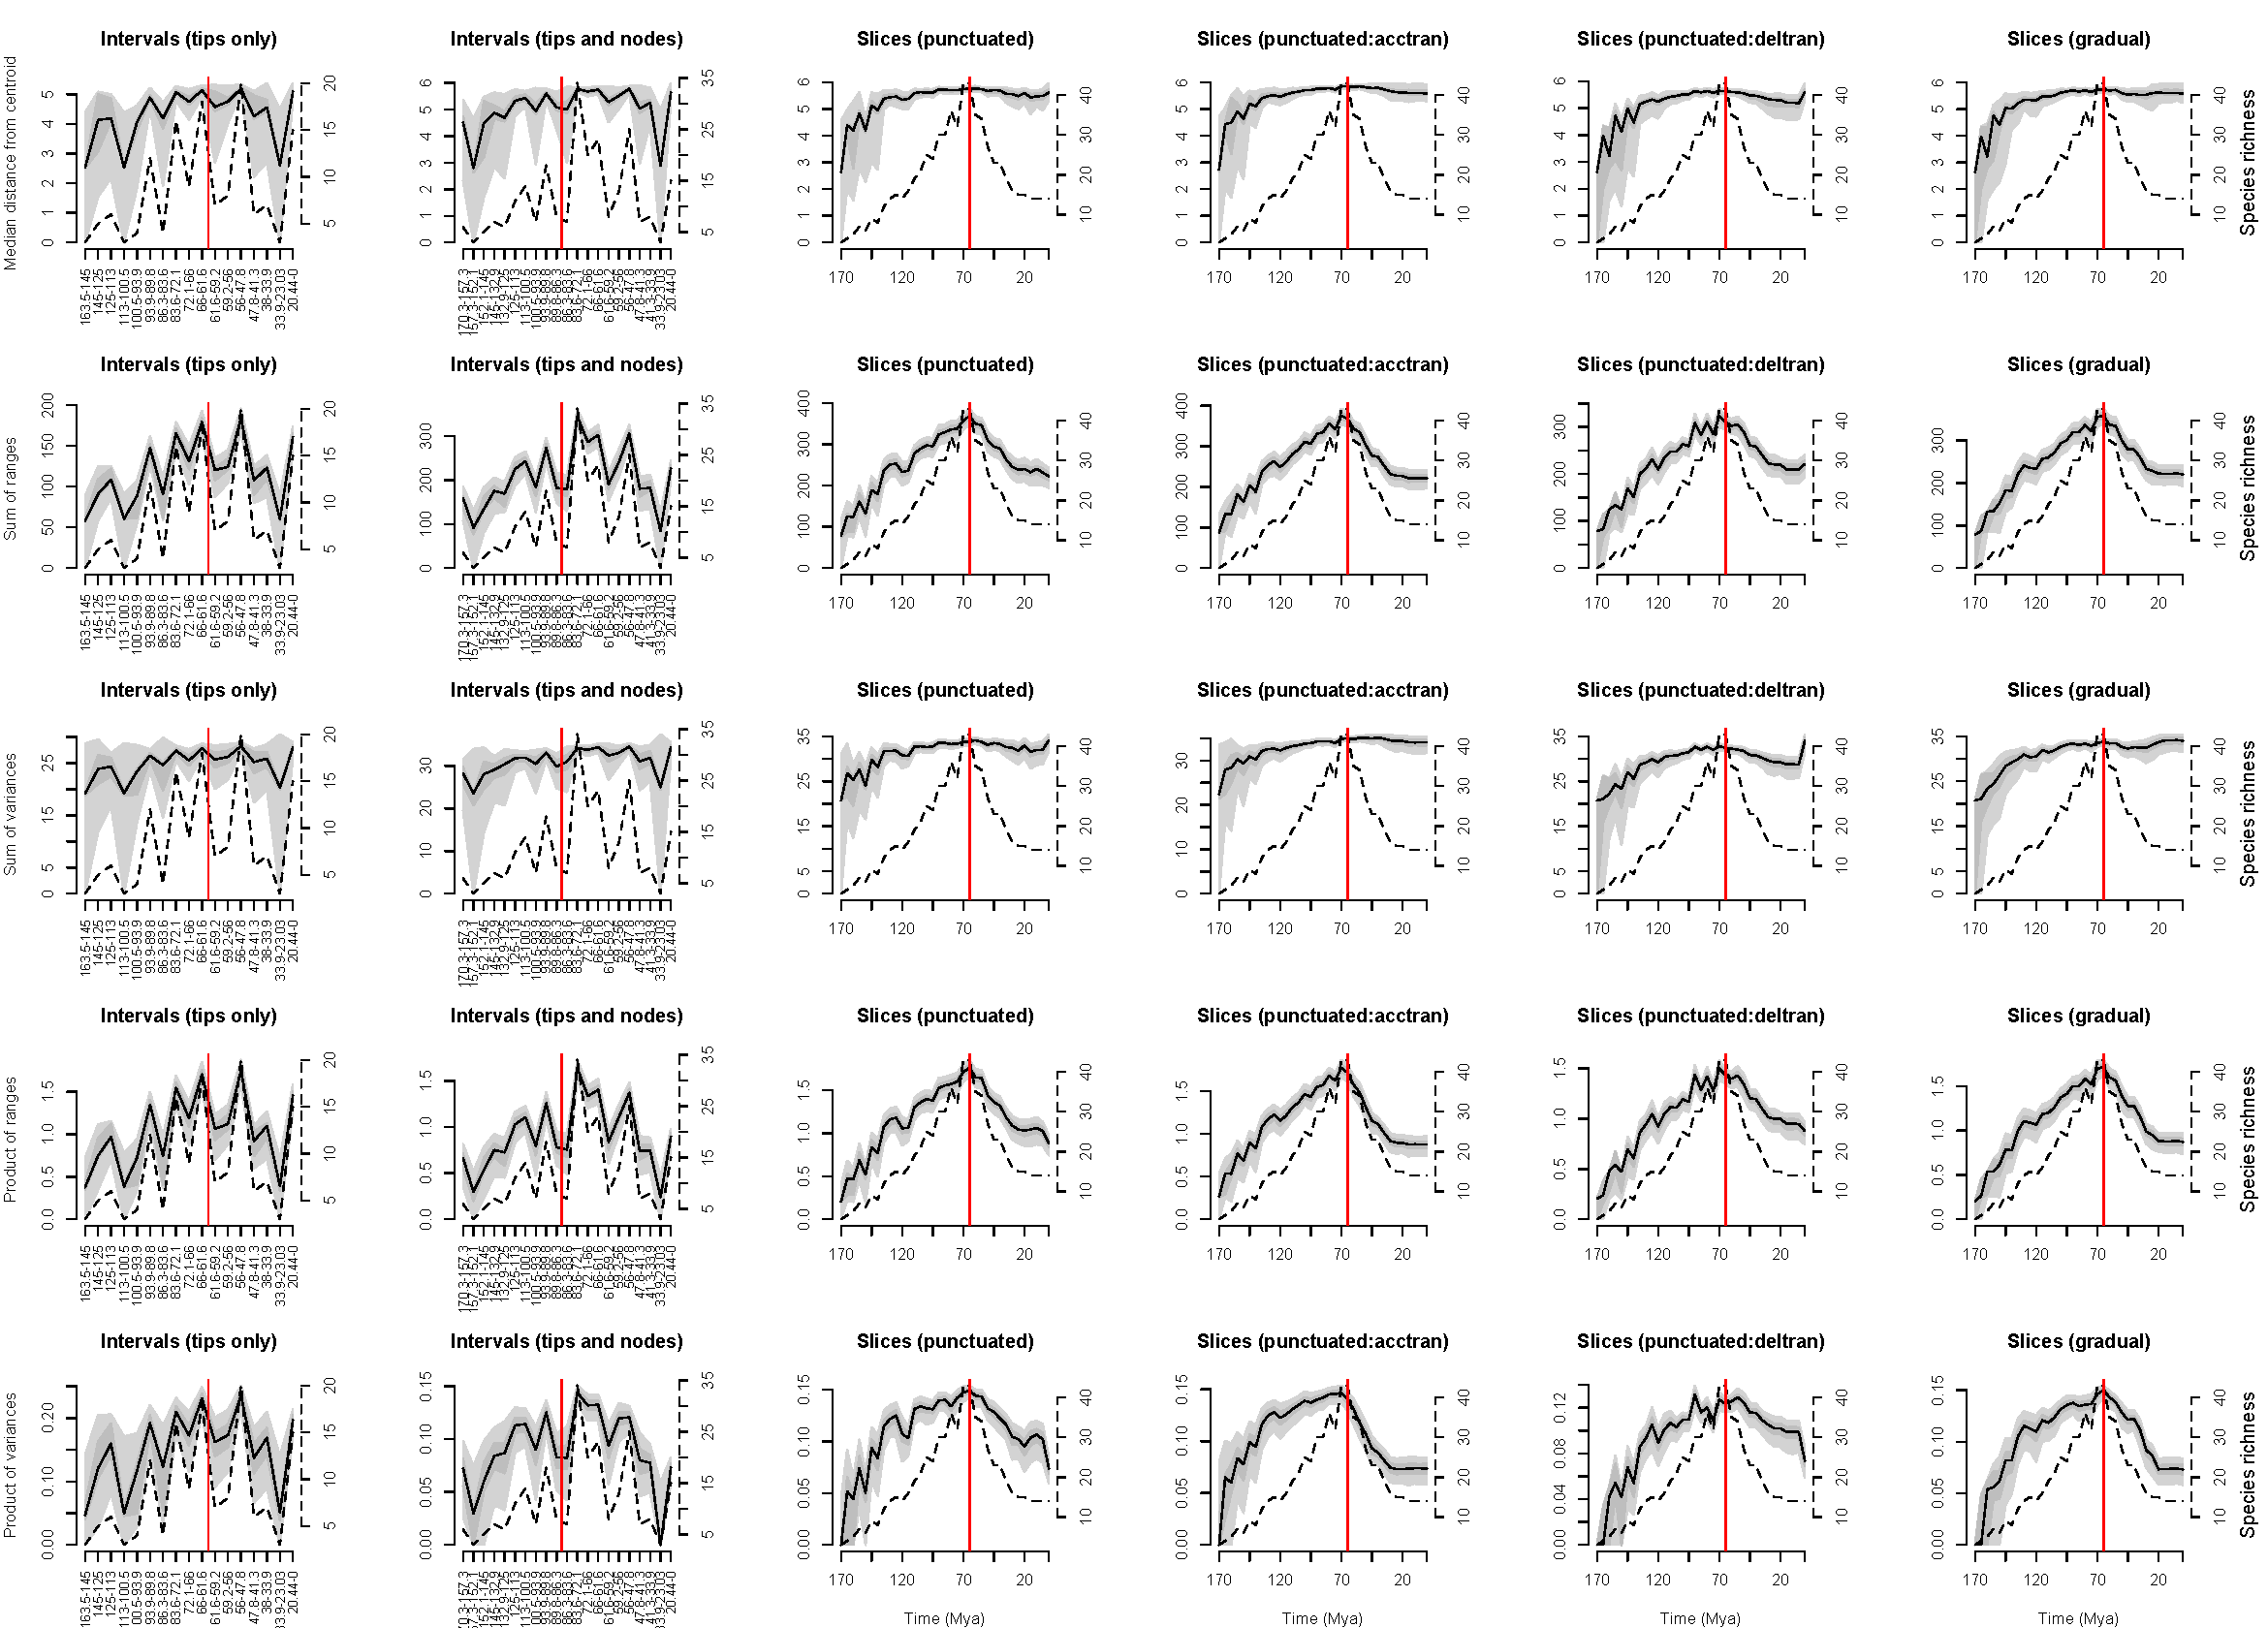
\includegraphics[width=\textwidth,height=\textheight,keepaspectratio]{Supplementaries/Figures/STD/Eutheria_all_methods.pdf}
\caption[Comparison of all the disparity metrics and all the time sampling methods for Eutheria]{Variations in disparity through time among Eutheria with different disparity measurements and methods for sampling disparity through time. The x axis represents time in millions of years before the present (Ma). The y axis represents disparity, measured as either the median distance between the centroid of the ordinated space and the tips/nodes in each time subsample, or the sum and product of ranges and variances of each axis of the cladisto-space. The solid black lines show the mean disparity estimated from 1000 bootstrapped pseudoreplicates and confidence intervals (CI) are represented by the grey polygons (50\% CI in dark grey and 95\% CI in light grey). The dashed line and the right hand axis represents the number of tips/nodes in each time slice. The red vertical line indicates the Cretaceous-Paleogene (K-Pg) boundary (66 Ma). Note that scale bars differ among panels.}
\label{Supp_disparity_all_Eutheria}
\end{figure}
\end{landscape}

\begin{landscape}
\begin{figure}[!htbp]
\centering
    \includegraphics[width=\textwidth,height=\textheight,keepaspectratio]{Supplementaries/Figures/STD/Mammaliaformes_all_methods_rarefied.pdf}
\caption[Comparison of all the disparity metrics and all the time sampling methods for Mammaliaformes (rarefied)]{Variations in disparity through time among Mammaliaformes with different disparity measurements and methods for sampling disparity through time (rarefied with three taxa for the intervals methods and eight taxa for the slices methods). The x axis represents time in millions of years before the present (Ma). The y axis represents disparity, measured as either the median distance between the centroid of the ordinated space and the tips/nodes in each time subsample, or the sum and product of ranges and variances of each axis of the cladisto-space. The solid black lines show the mean disparity estimated from 1000 bootstrapped pseudoreplicates and confidence intervals (CI) are represented by the grey polygons (50\% CI in dark grey and 95\% CI in light grey). The dashed line and the right hand axis represents the number of tips/nodes in each time slice. The red vertical line indicates the Cretaceous-Paleogene (K-Pg) boundary (66 Ma). Note that scale bars differ among panels.}
\label{Supp_disparity_all_Mammaliaformes_rarefied}
\end{figure}
\end{landscape}

\begin{landscape}
\begin{figure}[!htbp]
\centering
    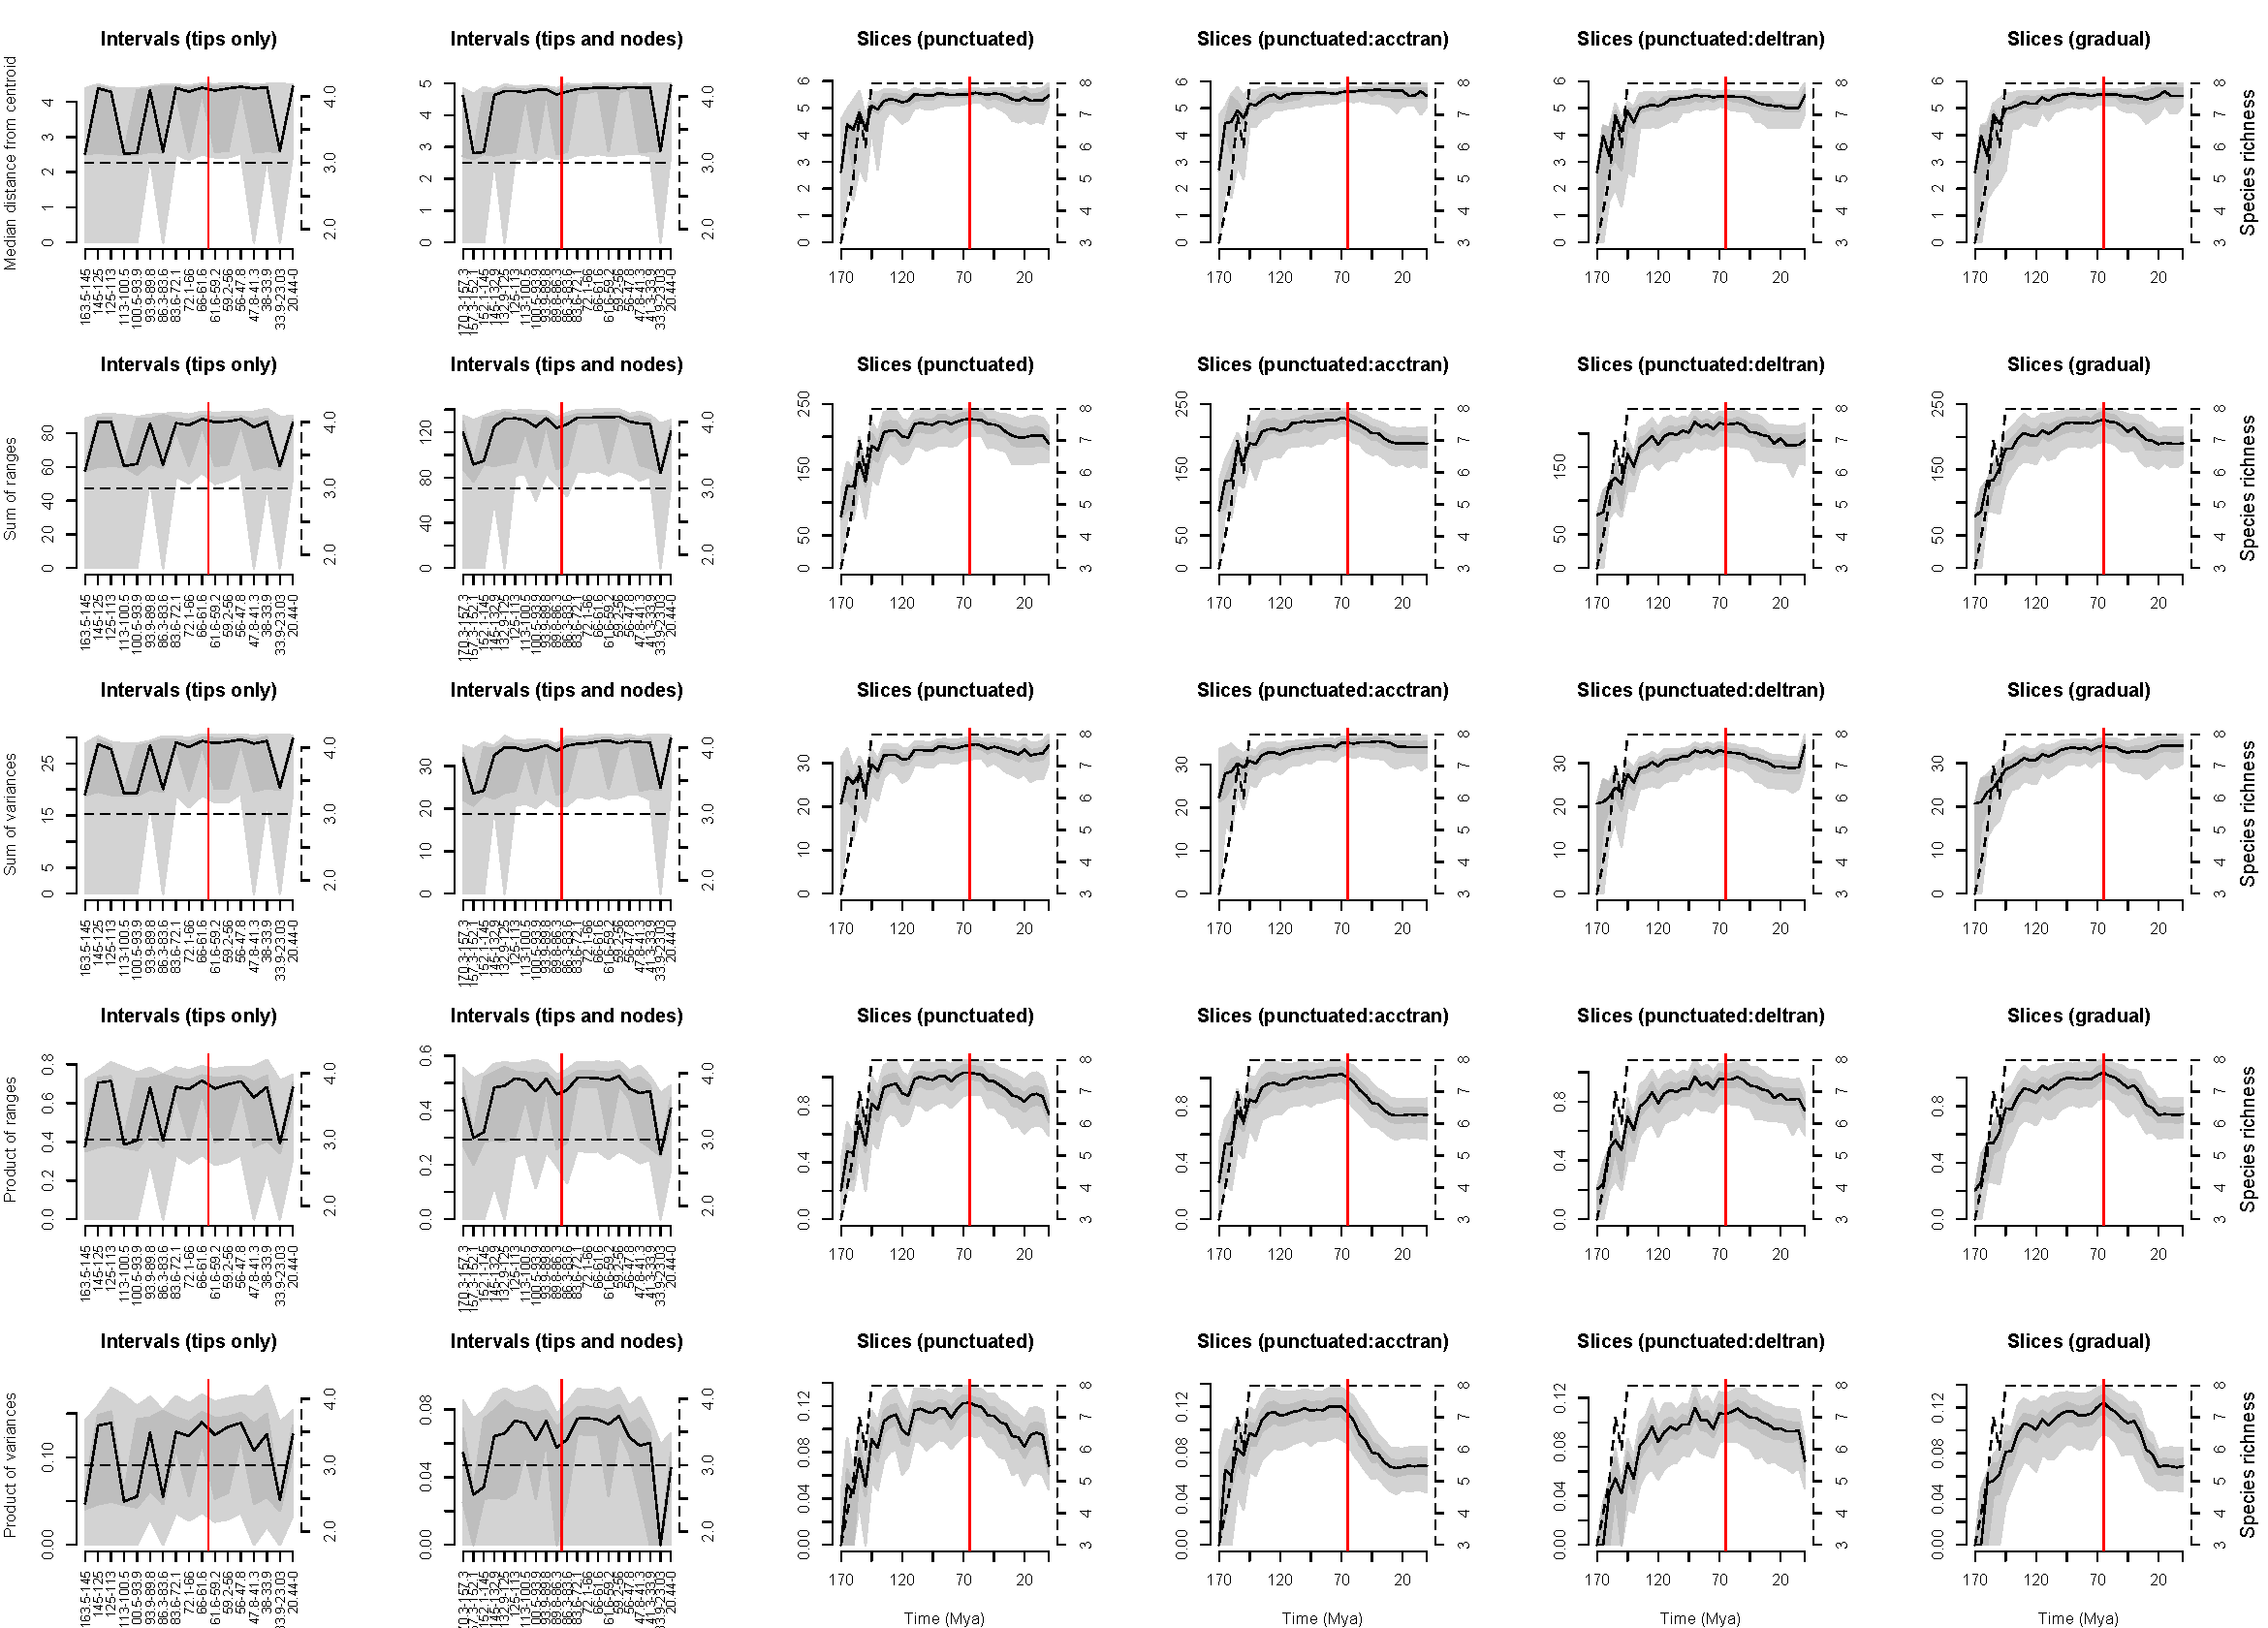
\includegraphics[width=\textwidth,height=\textheight,keepaspectratio]{Supplementaries/Figures/STD/Eutheria_all_methods_rarefied.pdf}
\caption[Comparison of all the disparity metrics and all the time sampling methods for Eutheria (rarefied)]{Variations in disparity through time among Eutheria  with different disparity measurements and methods for sampling disparity through time (rarefied with three taxa for the intervals methods and eight taxa for the slices methods). The x axis represents time in millions of years before the present (Ma). The y axis represents disparity, measured as either the median distance between the centroid of the ordinated space and the tips/nodes in each time subsample, or the sum and product of ranges and variances of each axis of the cladisto-space. The solid black lines show the mean disparity estimated from 1000 bootstrapped pseudoreplicates and confidence intervals (CI) are represented by the grey polygons (50\% CI in dark grey and 95\% CI in light grey). The dashed line and the right hand axis represents the number of tips/nodes in each time slice. The red vertical line indicates the Cretaceous-Paleogene (K-Pg) boundary (66 Ma). Note that scale bars differ among panels.}
\label{Supp_disparity_all_Eutheria_rarefied}

\end{figure}
\end{landscape}